\chapter{Analisador Léxico}
\label{cap:lexico}
Neste capítulo será descrita a implementação do Analisador Léxico. Esse componente do compilador é responsável por ler o arquivo fonte e transformá-lo em uma sequência de tokens.

\section{Definição dos Tokens}
\label{sec:lexicoDefinicaoTokens}
Inicialmente, foi necessário definir quais serão os tokens da linguagem nessa implementação. Com base, na gramática apresentada na seção \ref{sec:gramatica}, foi definida a seguinte lista de tokens:

Tokens Básicos: ROUTINE, BEGIN, END, DECLARE, INT, FLOAT, CHAR, IF, THEN, ELSE, REPEAT, UNTIL, WHILE, DO, READ, WRITE, NOT, OR, AND, ASSIGN, ADD, SUB, MUL, DIV, COMP\_EQ, COMP\_NE, COMP\_GT, COMP\_GE, COMP\_LT, COMP\_LE, OPEN\_BRACES, CLOSE\_BRACES, SEMICOLON, COMMA

Constantes: CONST\_INT, CONST\_FLOAT, CONST\_CHAR, CONST\_STRING

Identificadores: ID

Outros Tokens: END\_OF\_FILE, INVALID\_TOKEN, ERROR

\section{Estrutura do programa}
\label{sec:lexicoEstrutura}
Foi criada uma classe Token para representar os tokens da linguagem.
Essa classe possui um enum TokenType utilizado para armazenar o tipo de token que o objeto representa, com base na lista apresentada na seção \ref{sec:lexicoDefinicaoTokens}.
Para representar constantes, foi definida uma classe derivada de Token, chamada de ValueType.
Dessa classe foram derivadas as classes TokenConstInt, TokenConstFloat, TokenConstChar e TokenConstString, com cada objeto armazenando seu respectivo valor.
Finalmente, para Identificadores, foi criada a classe TokenId, derivada de Token, que armazena seu id e uma referência para o ValueType com seu respectivo valor.

Para navegar no arquivo fonte, foi criada uma classe FileHandler, que é responsável por abrir e ler o arquivo.
Essa classe também armazena um objeto do tipo struct chamado FilePosition, que indica a linha e a coluna atual do arquivo e também oferece uma função putback que retorna o último caractere lido para o buffer.

A implementação da tabela de símbolos foi realizada por meio da classe SymbolTable.
Ela armazena um unordered\_map (correspondente a um hash map) que relaciona o nome de um símbolo com seu respectivo objeto do tipo Token.
Ela implementa dois métodos, insertSymbol() e insertId(), que podem ser utilizados para inserir um novo token na tabela, ou para retornar o token já existente.

O Analisador Léxico em si foi implementado por meio de um parser recursivo descendente. Ele possui um método principal, getNextToken(), que retorna um ponteiro para o próximo Token lido.
Para evitar criar tokens de forma desnecessária, ele armazena um array com os tokens básicos, já que eles são imutáveis.
Ele também armazena um vetor com os ValueTokens que são criados.
Essa parte é necessária pois eles são alocados de forma dinâmica na memória e portanto é preciso armazenar uma referência para posteriormente liberar a memória, e, no caso dos ValueTypes, não se pode saber a tempo de compilação até em que momento eles serão utilizados.
O Analisador Léxico também armazena o FileHandler e a SymbolTable, para seu uso.
Ao se iniciar a execução, a tabela de símbolos é populada com as palavras reservadas da linguagem, pois dessa forma elas podem ser tratadas pelo Léxico como identificadores durante o processo de parsing do arquivo.

A seguir encontra-se o diagrama de classes do programa, no estilo UML:

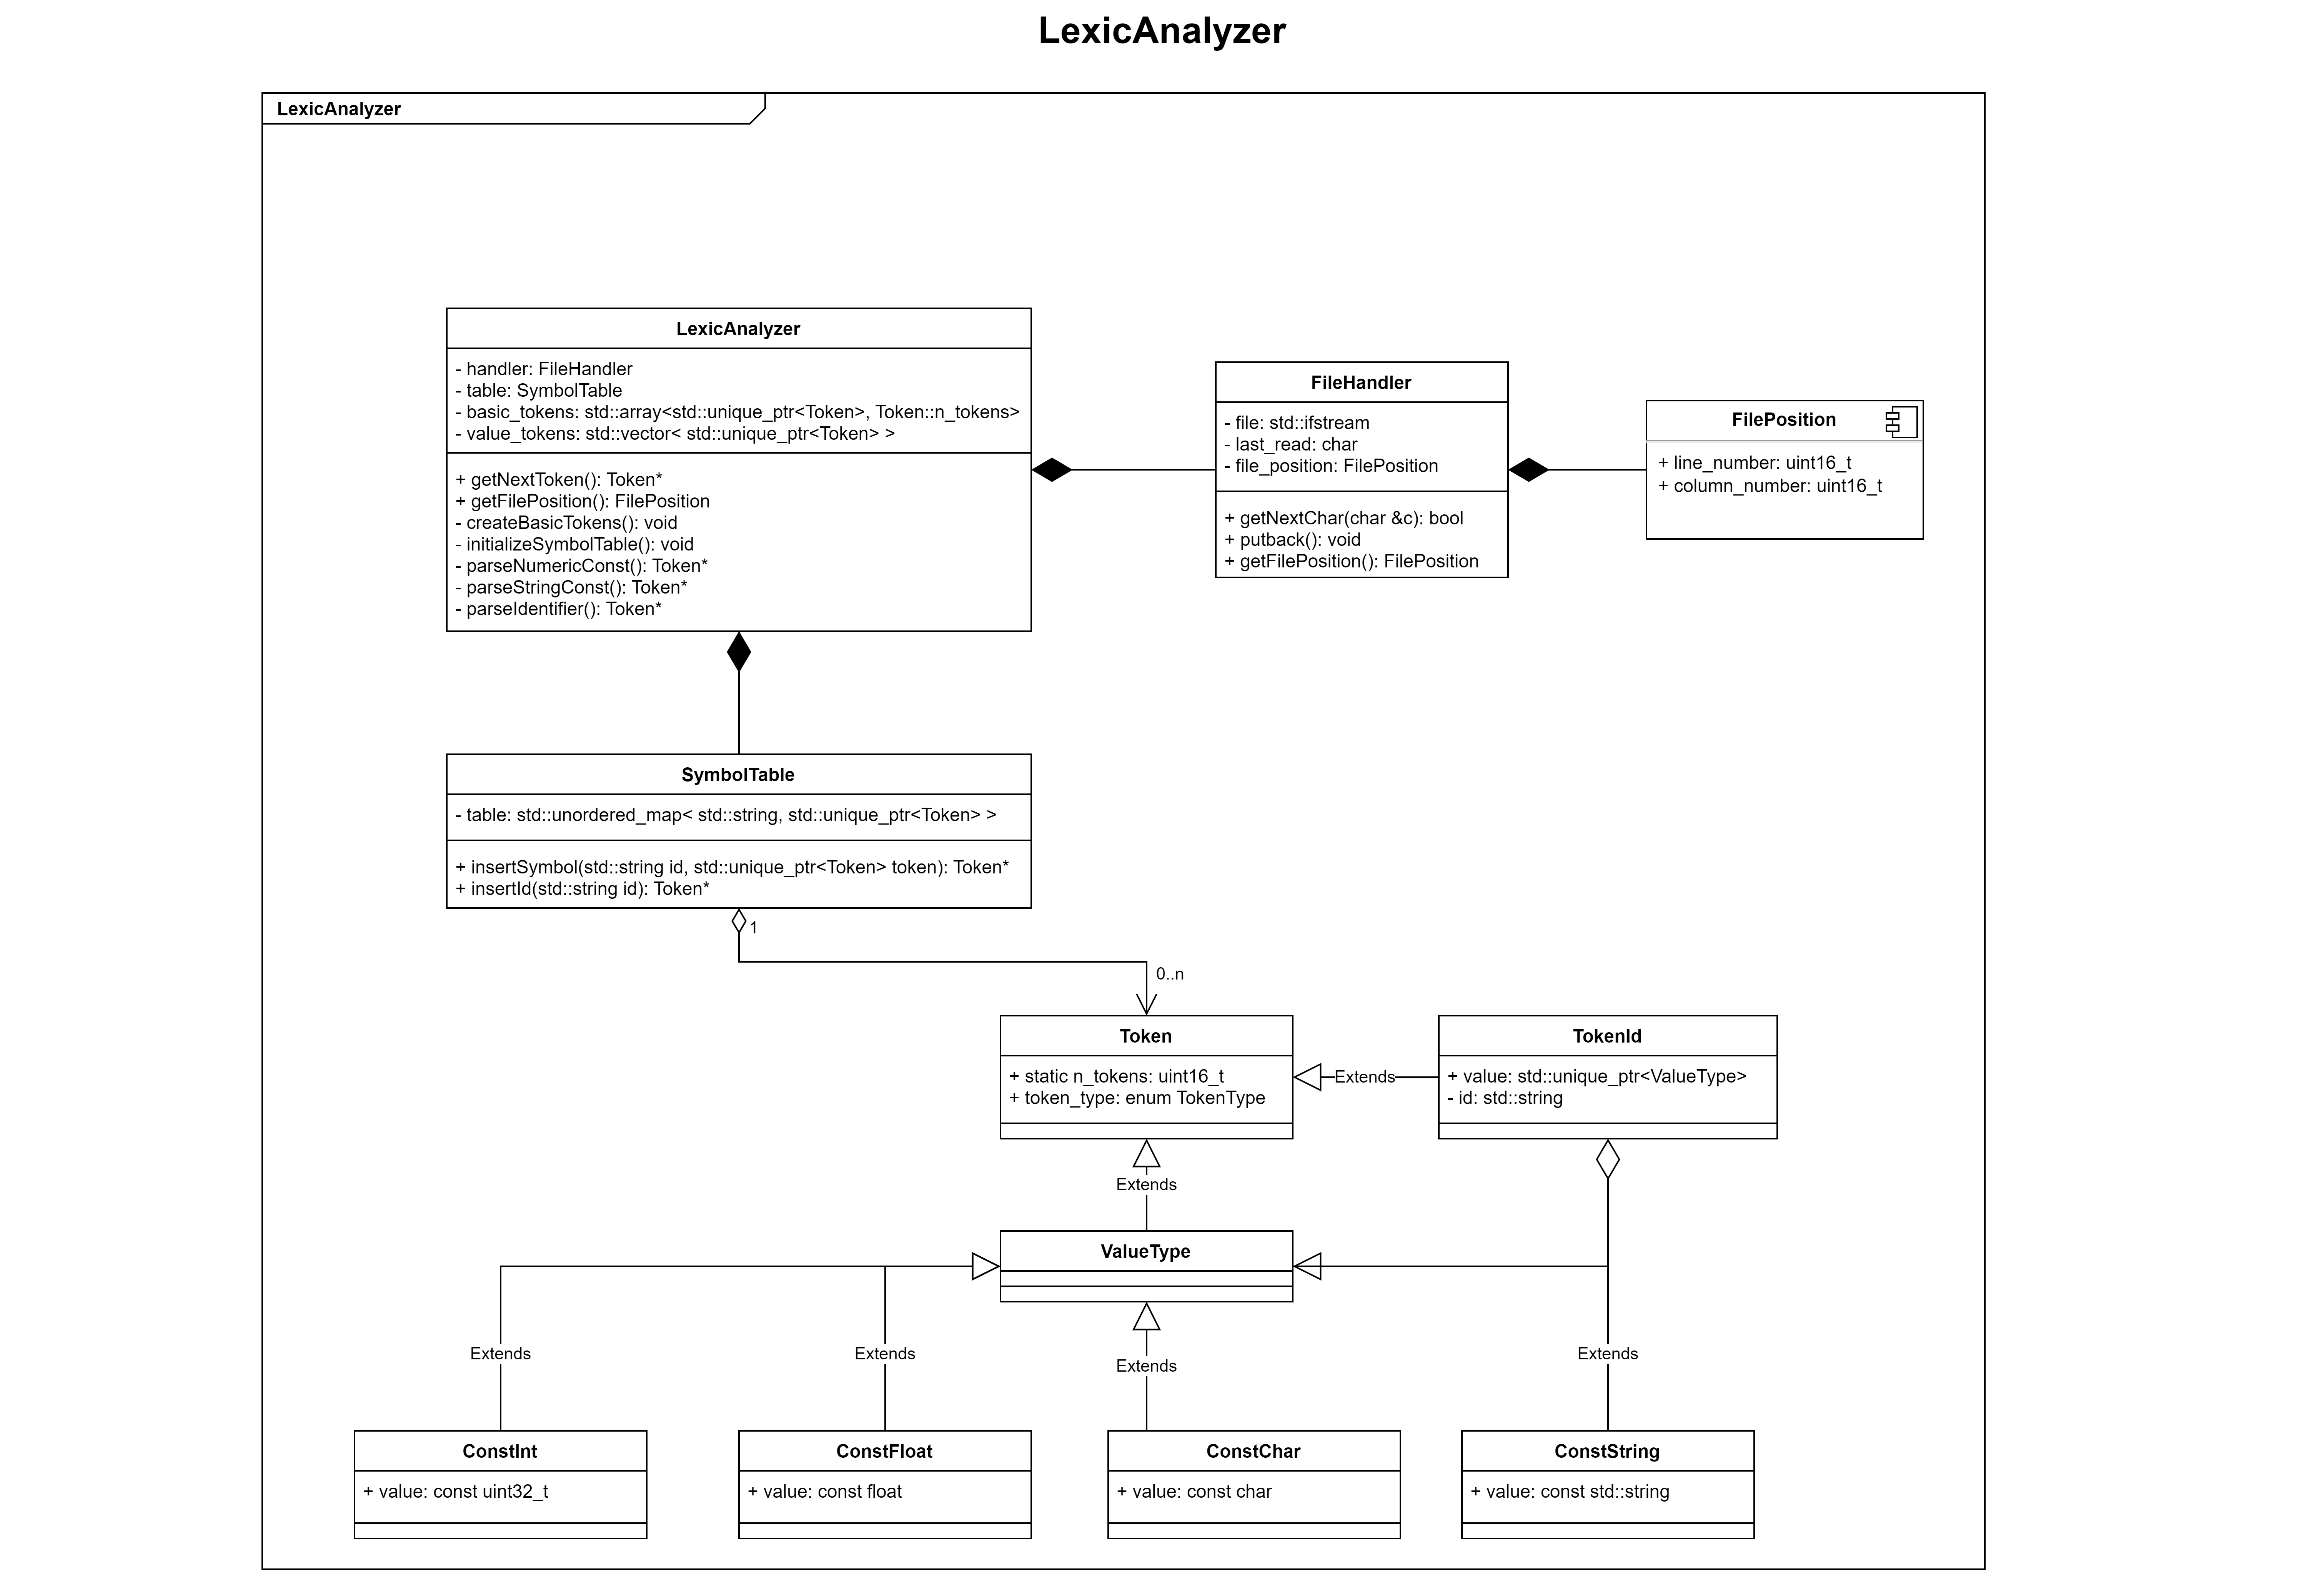
\includegraphics[width=\linewidth]{2-Imagens/Lexico-UML.png}

\section{Testes de validação}
\label{sec:lexicoTestes}

\subsection{Teste 01}
\label{subsec:lexicoTeste01}

\subsubsection{Código Original}
\verbatiminput{3-testes/lexico/1/original.txt}

\subsubsection{Código Corrigido}
\verbatiminput{3-testes/lexico/1/fixed.txt}

\subsection{Teste 02}
\label{subsec:lexicoTeste02}

\subsubsection{Código Original}
\verbatiminput{3-testes/lexico/2/original.txt}

\subsubsection{Código com Comentário Corrigido}
\verbatiminput{3-testes/lexico/2/fixedComment.txt}

\subsubsection{Código Corrigido}
\verbatiminput{3-testes/lexico/2/fixed.txt}

\subsection{Teste 03}
\label{subsec:lexicoTeste03}

\subsubsection{Código Original}
\verbatiminput{3-testes/lexico/3/original.txt}

\subsubsection{Código Corrigido}
\verbatiminput{3-testes/lexico/3/fixed.txt}

\subsection{Teste 04}
\label{subsec:lexicoTeste04}

\subsubsection{Código Original}
\verbatiminput{3-testes/lexico/4/original.txt}

\subsubsection{Código com String Corrigida}
\verbatiminput{3-testes/lexico/4/fixedString.txt}

\subsubsection{Código Corrigido}
\verbatiminput{3-testes/lexico/4/fixed.txt}

\subsection{Teste 05}
\label{subsec:lexicoTeste05}

\subsubsection{Código Original}
\verbatiminput{3-testes/lexico/5/original.txt}

\subsubsection{Código com String Corrigida}
\verbatiminput{3-testes/lexico/5/fixedString.txt}

\subsubsection{Código Corrigido}
\verbatiminput{3-testes/lexico/5/fixed.txt}

\subsection{Teste 06}
\label{subsec:lexicoTeste06}

\subsubsection{Código Original}
\verbatiminput{3-testes/lexico/6/original.txt}

\subsubsection{Código Corrigido}
\verbatiminput{3-testes/lexico/6/fixed.txt}

\subsection{Teste 07}
\label{subsec:lexicoTeste07}

\subsubsection{Código Original}
\verbatiminput{3-testes/lexico/7/original.txt}

\subsubsection{Código Corrigido}
\verbatiminput{3-testes/lexico/7/fixed.txt}